\documentclass[a4paper,12pt]{article}

%%% Размер шрифта
\usepackage[14pt]{extsizes}

%%% Поля
\usepackage[
	left=2cm,
	right=2cm,
	top=2cm,
	bottom=3cm,
	bindingoffset=0cm
]{geometry}

%%% Работа с русским языком
\usepackage{cmap}						% поиск в PDF
\usepackage{mathtext}					% русские буквы в формулах
\usepackage[T2A]{fontenc}				% кодировка
\usepackage[utf8]{inputenc}				% кодировка исходного текста
\usepackage[english,russian]{babel}		% локализация и переносы
\usepackage{indentfirst}
\frenchspacing

%%% Дополнительная работа с математикой
\usepackage{amsmath,amsfonts,amssymb,amsthm,mathtools}  % AMS

%%% Текст в колонки
\usepackage{multicol}

%%% Списки
\usepackage{enumitem}
\setlist{nosep, leftmargin=*}
\renewcommand{\labelenumi}{\arabic*)}

%%% Системы уравнений
\usepackage{cases}

%%% Таблицы
\usepackage{array}

%%% Рисунки
\usepackage{graphicx}
\usepackage{float}

%%% Точка в подписях к рисункам
\usepackage[labelsep=period]{caption}

%%% Список литературы
\bibliographystyle{bibliography_style/gost-numeric.bbx}
\usepackage[
	natbib = true,
	style = gost-numeric,
	sorting = none,
	backend = biber,
	language = autobib,
	autolang = other
]{biblatex}
\addbibresource{references.bib}

%%% Исправление символа номера при использовании gost-numeric.bbx
\usepackage{textcomp}
\DefineBibliographyStrings{russian}{number={\textnumero}}

%%% Гиперссылки
\usepackage[pdftex,unicode]{hyperref}

%%% Перенос знаков в формулах (по Львовскому)
\newcommand*{\hm}[1]{#1\nobreak\discretionary{}{\hbox{$\mathsurround=0pt #1$}}{}}


%%% Свои команды

\newcommand*{\No}{\textnumero}

\newcommand{\vect}[1]{\boldsymbol{#1}}
\newcommand{\vx}{{\vect{x}}}
\newcommand{\vn}{{\vect{n}}}

\newcommand{\half}{\cfrac{1}{2}}

\newcommand{\partt}[1]{\cfrac{\partial #1}{\partial t}}
\newcommand{\partx}[1]{\cfrac{\partial #1}{\partial x}}
\newcommand{\partxx}[1]{\cfrac{\partial^2 #1}{\partial x^2}}
\newcommand{\partvn}[1]{\cfrac{\partial #1}{\partial \vn}}

\newcommand{\partflt}[1]{\partial #1 / \partial t}
\newcommand{\partflx}[1]{\partial #1 / \partial x}
\newcommand{\partflxx}[1]{\partial^2 #1 / \partial x^2}
\newcommand{\partflvn}[1]{\partial #1 / \partial \vn}

\newcommand{\difftau}[1]{\cfrac{{#1}_j^{k + 1} - {#1}_j^k}{\tau}}
\newcommand{\diffhh}[1]{\cfrac{{#1}_{j + 1}^k - 2 {#1}_j^k + {#1}_{j - 1}^k}{h^2}}

\newcommand{\scalsq}[1]{\left( \nabla #1, \nabla #1 \right)}

\newcommand{\Natural}{{\mathbb{N}}}
\newcommand{\Real}{{\mathbb{R}}}
\newcommand{\bigO}{{\mathcal{O}}}
\newcommand{\clOmega}{{\overline{\Omega}}}

\newcommand{\norm}[1]{\| \, #1 \, \|}
\newcommand{\enorm}{{\| \cdot \|}}

\newcommand{\tabletopspace}{9mm}
\newcommand{\tablebottomspace}{3mm}

\newcommand{\tpoint}{{\text{.}}}
\newcommand{\tcomma}{{\text{,}}}
\newcommand{\tsemicolon}{{\text{;}}}

\newcommand{\unitm}{{\text{м}}}
\newcommand{\units}{{\text{с}}}
\newcommand{\unitJ}{{\text{Дж}}}
\newcommand{\unitC}{{\text{Кл}}}
\newcommand{\unitF}{{\text{Ф}}}

\newcommand{\forcehyphenation}{-\linebreak}


%%% Свои операторы
\DeclareMathOperator{\Div}{{div}}
\DeclareMathOperator{\Int}{{Int}}


%%% Оформление теорем

\theoremstyle{plain}
\newtheorem{theorem}{Теорема}
\newtheorem{proposition}{Утверждение}

\theoremstyle{remark}
\newtheorem{remark}{Замечание}


%%% Пояснение к меткам
% eq	-- equation
% cond	-- condition
% char	-- characteristic
% sch	-- scheme
% est	-- estimation
% exp	-- experiment
% fig	-- figure
% tab	-- table
% sec	-- section


%%% Описание препринта
\newcommand{\PreprintTitle}{
	Устойчивость стационарных решений модели развития канала электрического пробоя типа <<диффузной границы>>
}
\newcommand{\PreprintTitleEnglish}{
	Stability of stationary solutions of a diffuse interface model for electrical breakdown process
}
\newcommand{\PreprintAuthors}{
	А.С.~Пономарев, Е.В.~Зипунова, Е.Б.~Савенков
}
\newcommand{\PreprintAuthorsEnglish}{
	A.S.~Ponomarev, E.V.~Zipunova, E.B.~Savenkov
}


%%%%%%%%%%%%%%%%%%%%%%%%%%%%%%%%%%%%%%%%%%%%%%%%%%%%%%%%%%%%%%%%%%%%%%%%%%%%%%%%

\begin{document}

%%%%%%%%%%%%%%%%%%%%%%%%%%%%%%%%%%%%%%
\begin{titlepage}

\begin{center}
	РОССИЙСКАЯ АКАДЕМИЯ НАУК \\
	ОРДЕНА ЛЕНИНА \\
	ИНСТИТУТ ПРИКЛАДНОЙ МАТЕМАТИКИ \\
	имени М. В. КЕЛДЫША \\

	\vspace*{60mm}
	\Large{\PreprintAuthors} \\
	\vspace*{20mm}
	\textbf{\large \PreprintTitle} \\
	\vspace*{110mm}
	\Large{Москва, 2024}
	\vspace*{-50mm}
\end{center}

\end{titlepage}
%%%%%%%%%%%%%%%%%%%%%%%%%%%%%%%%%%%%%%%

\setcounter{page}{2}

\thispagestyle{empty}

\noindent \emph{\PreprintAuthors}, \PreprintTitle \\[3mm]
\textbf{Аннотация} \\
{
	\small
	Цель настоящей работы -- исследование качественных характеристик и численный анализ модели типа диффузной границы, описывающей развитие канала электрического пробоя в твердом диэлектрике. Проведен анализ устойчивости положений равновесия системы; установлены условия развития канала пробоя из малых возмущений неповрежденной среды. Построена и изучена разностная схема для задачи, дана содержательная оценка ее устойчивости. Полученные теоретические результаты подтверждены моделированием на компьютере. \\[3mm]
	\textbf{Ключевые слова:} модель типа диффузной границы, фазовое поле, устойчивость, электрический пробой. \\[5mm]
}
\begin{otherlanguage}{english}
\emph{\PreprintAuthorsEnglish}, \PreprintTitleEnglish \\[3mm]
\textbf{Abstract} \\
{
	\small
	The aim of the present work is to study qualitative characteristics and to perform a computational analysis of a diffuse interface model describing electrical breakdown process in a solid dielectric. Equilibrium solutions of the system are analysed. Conditions of small perturbations to cause development of a breakdown channel are found. A differential scheme for the problem is constructed and investigated, an informative estimate of its stability is given. The obtained theoretical results are validated by a computer simulation. \\[3mm]
	\textbf{Key words and phrases:} diffuse interface model, phase field, stability, electrical breakdown. \\[5mm]
}
\end{otherlanguage}

\clearpage

%!TEX root = ../main.tex

\section{Введение}

Электрический пробой~-- это явление резкого возрастания тока в диэлектрике при приложении электрического напряжения выше некоторого критического значения. Механизм разрушения диэлектрика под действием электрического поля сложен и многообразен: оно может иметь различные причины, характер развития, сопутствующие физические процессы \cite{vorobiev_dielectric_physics}.

Среди многообразия математических моделей, созданных для описания развития канала электрического пробоя, выделим предложенную в работе \cite{pitike_dielectric_breakdown} модель типа диффузной границы.

В настоящее время модели типа диффузной границы составляют целый класс подходов для решения задач в различных областях науки и техники. В частности, описанная в работе \cite{pitike_dielectric_breakdown} модель построена как формальное обобщение ранее известных моделей типа диффузной границы, применяемых в теории трещин.

Исследование и дальнейшее развитие упомянутой модели можно найти в работах \cite{zipunova_higher_codimension, zipunova_conservative, zipunova_thermomechanical, ponomarev_stability}. Основные положения метода диффузной границы в применении к моделированию развития канала электрического пробоя перечислены в работе \cite{ponomarev_stability}.

Модели типа диффузной границы используются для описания систем, в которых вещество может находиться в нескольких различных состояниях~-- фазах,~-- причем вещество в одной и той же фазе образует некоторые однородные области. В моделях типа диффузной границы распределение фаз вещества задается гладкой функцией $\phi$~-- фазовым полем,~-- которая в каждой области однородности близка к постоянной. Характерная толщина разделяющего слоя (<<диффузной границы>>) и, соответственно, скорость изменения~$\phi$ при переходе от одной фазы к другой определяется параметрами модели.

В работе \cite{zipunova_higher_codimension} проводится исследование свойства упомянутой модели развития канала электрического пробоя, которое можно назвать коразмерностью <<включений>>. Для задач теории трещин естественным будет двумерное включение (плоская трещина) в трехмерной среде вещества~-- в таком случае говорят, что коразмерность объекта равна 1. Обратим внимание, что, хотя исследуемая модель, как было сказано, получена на основе моделей из теории трещин, для нее характерным будет одномерное включение (канал пробоя), то есть имеющее коразмерность 2. В работе \cite{zipunova_higher_codimension} указано, что это может привести к нетривиальным последствиям, и предложено определенное обобщение исходной модели, которое предположительно делает ее более адекватной.

Суть обобщения состоит в формальном добавлении в уравнения модели двух слагаемых высших порядков с некоторыми коэффициентами. Целью настоящей работы является численная проверка поведения модели при различных значениях коэффициентов. Для этого ищется стационарное распределение фазового поля $\phi$ в нескольких характеристических случаях. Построение разностной схемы для задачи несет определенные сложности, связанные с необходимостью задать граничные условия на множествах коразмерности~2 и~3 в трехмерном пространстве. Предполагается, что точках этих множеств функция фазового поля $\phi$ имеет особенность.

Авторами применена модификация метода конечных объемов. Для части конфигураций обобщенной модели она позволила составить разнотную схему. Создана компьютерная программа, реализующая схему; проделаны расчеты, их результаты приведены в виде графиков. Для остальных конфигураций модели в процессе применения метода возникли фундаментальные проблемы, что позволяет выдвинуть гипотезу о некорректной постановке дифференциальной задачи в этих случаях.

%!TEX root = ../main.tex

\section{Постановка задачи и модель}
\label{sec:problem_and_model}

Приведем краткое описание математической модели, предложенной в работе \cite{pitike_dielectric_breakdown}. Подробное описание модели и физического смысла ее уравнений и параметров можно найти в работе \cite{ponomarev_stability}.

Рассматривается ограниченная область пространства $\Omega \subset \Real^3$. Распределение фаз вещества в ней задается гладкой функцией $\phi: \Omega \times [0, +\infty)_t \hm \to [0, 1], \; \phi(\vx, t)$~-- фазовым полем; вещество может находиться в одной из двух фаз: $\phi \approx 1$~-- <<неповрежденное>>, $\phi \approx 0$~-- <<полностью разрушенное>> (то есть относящееся к каналу пробоя),~-- а также в промежуточных состояниях в зоне диффузной границы.

Диэлектрическую проницаемость среды $\epsilon$ предлагается описать следующей формулой:
\begin{equation}
	\epsilon(\vx, t) = \epsilon[\phi] = \cfrac{\epsilon_0(\vx)}{f(\phi(\vx, t)) + \delta} \tpoint
	\label{eq:epsilon}
\end{equation}
Здесь $\epsilon_0(\vx)$~-- диэлектрическая проницаемость неповрежденной среды, $f(\phi) \hm = 4\phi^3 - 3\phi^4$~-- интерполирующая функция, $0 < \delta \ll 1$~-- регуляризующий параметр.

Помимо фазового поля $\phi$, состояние системы описывает также функция $\Phi: \Omega \times [0, +\infty)_t \to \Real, \; \Phi(\vx, t)$~-- потенциал электрического поля.

Постулируется следующее выражение для свободной энергии системы $\Pi$:
\begin{gather*}
	\Pi = \int \limits_\Omega \pi d \vx \tcomma \\
	\pi = -\half \epsilon[\phi] \scalsq{\Phi} + \Gamma \cfrac{1 - f(\phi)}{l^2} + \cfrac{\Gamma}{4} \scalsq{\phi} \tpoint
\end{gather*}
Здесь $\Gamma > 0, \; l > 0$~-- числовые параметры модели, константы.

Постулируются два уравнения, определяющие динамику системы:
\begin{equation*}
\begin{cases}
	\cfrac{\delta \Pi}{\delta \Phi} = 0 \tsemicolon \\[3mm]
	\cfrac{1}{m} \partt{\phi} = -\cfrac{\delta \Pi}{\delta \phi} \tpoint
\end{cases}
\end{equation*}
Здесь константа $m > 0$~-- числовой параметр модели, называемый подвижностью. Говоря нестрого, согласно первому уравнению электрический потенциал $\Phi$ распределяется так, чтобы свободная энергия была минимальной; согласно второму~-- фазовое поле $\phi$ с определенной скоростью стремится к тому, чтобы свободная энергия была минимальной.

Отыскав явно вариационные производные в двух уравнениях выше, получим следующую систему уравнений:
\begin{numcases}{}
	\Div(\epsilon[\phi] \nabla \Phi) = 0 \tsemicolon
	\label{eq:Phi} \\
	\cfrac{1}{m} \partt{\phi} = \half \epsilon'(\phi) \scalsq{\Phi} + \cfrac{\Gamma}{l^2} f'(\phi) + \half \Gamma \triangle \phi \tpoint
	\label{eq:phi}
\end{numcases}
Здесь $(\cdot)' \equiv (\cdot)_\phi'$. Система состоит из двух уравнений: на $\phi$ и $\Phi$ соответственно; система связная, второе уравнение нелинейное, является уравнением типа Аллена--Кана.

%!TEX root = ../main.tex

\section{Теоретическое исследование: \\ анализ положений равновесия}
\label{sec:theoretical_analysis}

При определенных условиях электрический пробой может развиваться из малых возмущений свойств неповрежденной среды. Для отыскания этих условий исследуем положения равновесия уравнения \eqref{eq:one_dim} вида $\phi(x, t) \equiv C,$ $C \in [0, 1]$ (то есть $\phi$ постоянна и во времени, и в пространстве).

Приведем формулы для производных $f(\phi)$ и $\epsilon(\phi)$ (последнее задано выражением \eqref{eq:epsilon}):
$$f(\phi) = 4 \phi^3 - 3 \phi^4 \tsemicolon \quad f'(\phi) = 12 \phi^2 - 12 \phi^3 \tsemicolon \quad f''(\phi) = 24 \phi - 36 \phi^2 \tpoint$$
$$\epsilon'_f = \cfrac{-\epsilon_0}{(f(\phi) + \delta)^2} \tsemicolon \quad \epsilon''_{ff} = \cfrac{2 \epsilon_0}{(f(\phi) + \delta)^3} \tsemicolon$$
откуда:
\begin{equation}
	\epsilon'(\phi) = \epsilon'_f \cdot f' = \cfrac{-\epsilon_0 f'(\phi)}{(f(\phi) + \delta)^2} \tsemicolon
	\label{eq:epsilon_phi}
\end{equation}
\begin{equation}
	\epsilon''(\phi) = \epsilon''_{ff} \cdot (f')^2 + \epsilon'_f \cdot f'' = \epsilon_0 \cfrac{2 (f'(\phi))^2 - f''(\phi)(f(\phi) + \delta)}{(f(\phi) + \delta)^3} \tpoint
	\label{eq:epsilon_phi_phi}
\end{equation}

Подставим решение $\phi(x, t) \equiv C$ в уравнение \eqref{eq:one_dim}, получим:
\begin{equation}
	0 = \half K_\Phi^2 \epsilon'(C) + \cfrac{\Gamma}{l^2} f'(C) \tpoint
	\label{eq:equilibrium}
\end{equation}
Отсюда с учетом выражения \eqref{eq:epsilon_phi} имеем:
$$f'(C) \left( \cfrac{\Gamma}{l^2} - \half K_\Phi^2 \cfrac{\epsilon_0}{(f(C) + \delta)^2} \right) = 0 \tpoint$$
Рассмотрим сначала случай $f'(C) = 0$: имеем $f'(C) = 12C^2 (1 - C) = 0$, следовательно, $C \in \{0, 1\}$. Значит, $\phi \equiv 0$ и $\phi \equiv 1$ -- положения равновесия.

Пусть теперь $C \neq 0, 1$. Тогда
$$\cfrac{\Gamma}{l^2} = \cfrac{K_\Phi^2 \epsilon_0}{2 (f(C) + \delta)^2} \quad \text{и} \quad f(C) + \delta = K_\Phi l \sqrt{\cfrac{\epsilon_0}{2 \Gamma}} \tpoint$$
$f(C) \in [0, 1]$, к тому же $f(\phi)$ строго возрастает, поэтому если $K_\Phi l \sqrt{\epsilon_0 / (2 \Gamma)} \hm \in (\delta, 1 + \delta)$, то уравнение \eqref{eq:equilibrium} имеет отличный от $0$ и $1$ третий корень
\begin{equation}
	C_3 = f^{-1} \left( K_\Phi l \sqrt{\cfrac{\epsilon_0}{2 \Gamma}} - \delta \right) \tpoint
	\label{eq:equilibrium_third}
\end{equation}
В противном случае у уравнения \eqref{eq:equilibrium} корня только два.

Итак, число положений равновесия зависит от выполнения условия
\begin{equation}
	\delta^2 < \cfrac{K_\Phi^2 l^2 \epsilon_0}{2 \Gamma} < (1 + \delta)^2 \tpoint
	\label{cond:equilibriums_number}
\end{equation}
Немного позже станет ясна его связь со свойствами положений равновесия $\phi \equiv 0$ и $\phi \equiv 1$ и всего уравнения \eqref{eq:one_dim} в целом.

Перейдем теперь к анализу устойчивости положений равновесия.

Пусть $\phi(x, t)$ -- некоторое решение уравнения \eqref{eq:one_dim}, $\delta \phi(x, t)$ -- возмущение. Запишем уравнение \eqref{eq:one_dim} для возмущенного решения $\phi + \delta \phi$:
$$\cfrac{1}{m} \partt{(\phi + \delta \phi)} = \half K_\Phi^2 \epsilon'(\phi + \delta \phi) + \cfrac{\Gamma}{l^2} f'(\phi + \delta \phi) + \half \Gamma \partxx{(\phi + \delta \phi)} \tcomma$$
откуда:
\begin{multline*}
	\cfrac{1}{m} \left( \partt{\phi} + \partt{(\delta \phi)} \right) = \half K_\Phi^2 [\epsilon'(\phi) + \epsilon''(\phi) \delta \phi + o(1) \delta \phi] + \\ + \cfrac{\Gamma}{l^2} [f'(\phi) + f''(\phi) \delta \phi + o(1) \delta \phi] + \half \Gamma \left( \partxx{\phi} + \partxx{(\delta \phi)} \right) \tpoint
\end{multline*}
С учетом того, что $\phi$ -- решение, перейдем к
$$\cfrac{1}{m} \partt{(\delta \phi)} = \half K_\Phi^2 [\epsilon''(\phi) + o(1)] \delta \phi + \cfrac{\Gamma}{l^2} [f''(\phi) + o(1)] \delta \phi + \half \Gamma \partxx{(\delta \phi)} \tpoint$$
Линеаризуем (отбросим бесконечно малые). Получим уравнение на возмущение
\begin{equation}
	\cfrac{1}{m} \partt{(\delta \phi)} = \left(\half K_\Phi^2 \epsilon''(\phi) + \cfrac{\Gamma}{l^2} f''(\phi) \right) \delta \phi + \half \Gamma \partxx{(\delta \phi)} \tpoint
	\label{eq:variation}
\end{equation}

Часть дальнейшего анализа удобно провести в общем виде, для уравнения
\begin{equation}
	\partt{(\delta \phi)} = A \delta \phi + B \partxx{(\delta \phi)} \tcomma
	\label{eq:variation_common}
\end{equation}
где $A$ и $B$ -- некоторые постоянные, причем $B > 0$.

Подставим в уравнение \eqref{eq:variation_common} $\delta \phi = e^{\alpha t} \sin(\omega x)$, то есть некоторую экспоненциально растущую или убывающую во времени (в зависимости от знака $\alpha$) гармонику, и получим уравнение относительно параметров возмущения:
$$\alpha e^{\alpha t} \sin(\omega x) = A e^{\alpha t} \sin(\omega x) - B \omega^2 e^{\alpha t} \sin(\omega x) \tcomma$$
откуда:
\begin{equation}
	\alpha = A - B \omega^2 \tpoint
	\label{eq:exponent_coefficient}
\end{equation}

Объединим три части рассуждения. Для уравнения \eqref{eq:one_dim} рассмотрим положение равновесия $\phi \equiv C$. Прибавим к нему возмущение $\delta \phi$; применим к $\delta \phi$ уравнение \eqref{eq:variation}, в $\epsilon''$ и $f''$ подставим $\phi = C$. Полученное уравнение имеет вид~\eqref{eq:variation_common}. В зависимости от значения коэффициента
$$A = \half K_\Phi^2 \epsilon''(C) + \cfrac{\Gamma}{l^2} f''(C)$$
возможно три случая.
\begin{enumerate}[label=\arabic*.]
	\item $A > 0$. При $\omega^2 \in [0, A / B)$ верно $\alpha > 0$, то есть существуют возмущения $\delta \phi$, возрастающие во времени. Значит, положение равновесия $\phi \equiv C$ неустойчивое.
	\item $A < 0$. Для любого $\omega$ выполняется $\alpha \leqslant A < 0$. Любое возмущение $\delta \phi$ на отрезке $[0, W]_x$ можно представить в виде интеграла Фурье по гармоникам, все они убывают не медленнее гармоники $\omega = 0$. Значит, положение равновесия $\phi \equiv C$ устойчивое.
	\item $A = 0$. Рассуждаем аналогично случаю $A < 0$, однако здесь возможны сколь угодно медленно убывающие гармоники (со сколь угодно малым $\alpha$). Этот случай соответствует нейтральному равновесию. Здесь проведенного анализа с линеаризацией недостаточно; пояснение будет дано позже.
\end{enumerate}

Рассмотрим положение равновесия $\phi \equiv 0$. Имеем $f''(0) = 0, \; \epsilon''(0) = 0$ (см. выражение \eqref{eq:epsilon_phi_phi}); получаем $A = 0$. Этот случай требует более глубокого анализа, назвать тип положения равновесия мы пока не можем.

Рассмотрим положение равновесия $\phi \equiv 1$. Здесь $f''(0) = -12, \; \epsilon''(0) \hm = 12 \epsilon_0 / (1 + \delta)^2$ (см. выражение \eqref{eq:epsilon_phi_phi}); получаем:
$$A = \half K_\Phi^2 \epsilon''(C) + \cfrac{\Gamma}{l^2} f''(C) = \cfrac{6 K_\Phi^2 \epsilon_0}{(1 + \delta)^2} - \cfrac{12 \Gamma}{l^2} \tpoint$$
Положение равновесия устойчиво при условии $A < 0$, то есть при
\begin{equation}
	\cfrac{K_\Phi^2 l^2 \epsilon_0}{2 \Gamma} < (1 + \delta)^2 \tpoint
	\label{cond:equilibrium_1_stable}
\end{equation}
Найдем $\omega_0$, при котором в случае неустойчивого положения равновесия возрастающие гармоники сменяются убывающими. Для этого рассмотрим выражение \eqref{eq:exponent_coefficient} с $\alpha = 0, \; B = \Gamma / 2$ и приведенным выше $A$. Получим:
$$0 = \cfrac{6 K_\Phi^2 \epsilon_0}{(1 + \delta)^2} - \cfrac{12 \Gamma}{l^2} - \cfrac{\Gamma}{2} \omega_0^2 \tcomma$$
откуда:
$$\omega_0 = 2 \sqrt{\cfrac{3 K_\Phi^2 \epsilon_0}{\Gamma (1 + \delta)^2} - \cfrac{6}{l^2}} \tpoint$$

Заметим, что условие \eqref{cond:equilibrium_1_stable} есть правое неравенство из условия \eqref{cond:equilibriums_number}. Чтобы объяснить это и сформировать полную картину происходящего, взглянем на положения равновесия немного под другим углом.

Решая уравнение \eqref{eq:equilibrium}, мы искали нули функции 
\begin{equation}
	\chi(\phi) = \half K_\Phi^2 \epsilon'(\phi) + \cfrac{\Gamma}{l^2} f'(\phi) \tpoint
	\label{eq:equilibruim_characteristic}
\end{equation}
Следовательно, любому положению равновесия $\phi \equiv C$ однозначно соответствует ноль~$C$ функции $\chi(\phi)$. Из вывода уравнения \eqref{eq:variation} на возмущение следует, что в его правой части при $\delta \phi$ стоит коэффициент $\chi'(\phi)$. После, проводя анализ уравнения \eqref{eq:variation_common} для положения равновесия $\phi \equiv C$, мы рассматривали случаи в зависимости от знака коэффициента $A$, который, как оказалось, равен $\chi'(C)$.

Подведем итог рассуждениям. Функция $\chi(\phi)$, определенная форму\forcehyphenation лой~\eqref{eq:equilibruim_characteristic}, гладкая на отрезке $[0, 1]$. Она имеет нули $0$ и $1$, а также при условии \eqref{cond:equilibriums_number} -- третий ноль в некоторой точке $C_3 \in (0, 1)$. Положения равновесия $\phi \equiv C$ однозначно соответствуют нулям $\chi(\phi)$. Вопрос их устойчивости сводится к отысканию знака $\chi'(\phi)$ в нулях: положительная $\chi'$ -- неустойчивое равновесие, отрицательная $\chi'$ -- устойчивое.

Теперь стало понятно, почему в случае нулевой $\chi'$ (как в точке $\phi = 0$) недостаточно анализа с линеаризацией уравнения на возмущение. Интуитивно понятно, что в случае нулевой первой производной нужно рассмотреть первую ненулевую производную высшего порядка; возрастание $\chi$ будет означать неустойчивое равновесие, убывание -- устойчивое.

В завершение докажем, что $\chi(\phi)$ в нуле $C_3 \in (0, 1)$ (в случае его существования) имеет ненулевую производную. Имеем:
$$\chi(C_3) = f'(C_3) \left( \cfrac{\Gamma}{l^2} - \cfrac{K_\Phi^2 \epsilon_0}{2 (f(C_3) + \delta)^2} \right) = 0 \tpoint$$
Учитывая, что $f'(C_3) \ne 0$, получим:
$$\cfrac{\Gamma}{l^2} - \cfrac{K_\Phi^2 \epsilon_0}{2 (f(C_3) + \delta)^2} = 0 \tpoint$$
Тогда:
$$\chi'(\phi)|_{C_3} = f'(C_3) \left( \cfrac{\Gamma}{l^2} - \cfrac{K_\Phi^2 \epsilon_0}{2 (f(\phi) + \delta)^2} \right) ' \bigg|_{C_3} = (f'(C_3))^2 \cfrac{K_\Phi^2 \epsilon_0}{(f(C_3) + \delta)^3} \ne 0 \tpoint$$

Теперь можно провести исчерпывающий разбор случаев поведения $\chi(\phi)$ в своих нулях. Как видно из условий \eqref{cond:equilibriums_number} и \eqref{cond:equilibrium_1_stable}, оно определяется величиной
\begin{equation}
	\xi = \cfrac{K_\Phi^2 l^2 \epsilon_0}{2 \Gamma} \tpoint
	\label{char:equilibriums}
\end{equation}

Вначале рассмотрим случай $0 \leqslant \xi < \delta^2$. Нули $\chi(\phi)$: $0$, $1$; $\chi'(0) = 0, \; \chi'(1) \hm < 0$. Поведение функции $\chi(\phi)$ схематично изображено на рис. \ref{fig:equilibriums_case_1}. Положения равновесия: $\phi \equiv 0$ неустойчивое, $\phi \equiv 1$ устойчивое. Эту конфигурацию условно назовем случаем <<слабого электрического напряжения>>. Интуитивно конфигурация означает, что при фиксированных прочих параметрах электрическое поле мало настолько, что даже близкая к полностью разрушенной среда $\phi \approx 0$ со временем <<восстанавливается>> до $\phi \approx 1$.

Рассмотрим теперь случай $\delta^2 < \xi < (1 + \delta)^2$. Нули $\chi(\phi)$: $0$, $C_3$ (см. выражение~\eqref{eq:equilibrium_third}), $1$; $\chi'(0) = 0, \; \chi'(1) < 0; \; \chi'(C_3) > 0$ (из гладкости $\chi$). Поведение функции $\chi(\phi)$ схематично изображено на рис. \ref{fig:equilibriums_case_2}. Положения равновесия: $\phi \equiv 0$ устойчивое, $\phi \equiv C_3$ неустойчивое, $\phi \equiv 1$ устойчивое. Такую конфигурацию условно назовем случаем <<среднего электрического напряжения>>. Интуитивно конфигурация означает, что при достаточно близких к $0$ значениях $\phi$ среда <<разрушается>> до $0$, при достаточно близких к $1$ -- <<восстанавливается>> до $1$; посередине же, <<на границе>>, -- неустойчивое равновесие.

Наконец, рассмотрим случай $(1 + \delta)^2 < \xi$. Нули $\chi(\phi)$: $0$, $1$; $\chi'(0) = 0,$ $\chi'(1) > 0$. Поведение функции $\chi(\phi)$ схематично изображено на рис. \ref{fig:equilibriums_case_3}. Положения равновесия: $\phi \equiv 0$ устойчивое, $\phi \equiv 1$ неустойчивое. Эту конфигурацию условно назовем случаем <<сильного электрического напряжения>>. Интуитивно конфигурация означает, что электрическое поле достаточно сильно, чтобы сколь угодно близкую к неповрежденной среду $\phi \approx 1$ <<разрушить>> до $\phi \approx 0$. Именно в этом случае электрический пробой развивается из малых возмущений свойств неповрежденной среды.

Во всех трех случаях устойчивость положения равновесия $\phi \equiv 0$ определяется по производной высшего порядка из вида функции $\chi(\phi)$.

\begin{figure}[!tp]
	\centering
	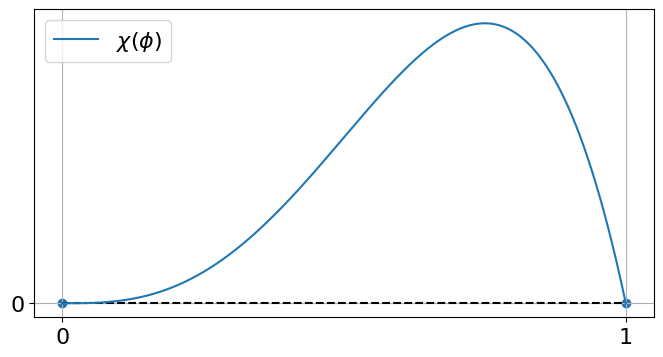
\includegraphics[width=0.77\textwidth]{figures/equilibriums_case_1.png}
	\vspace{-0.3cm}
	\caption{Поведение функции $\chi(\phi)$, случай <<слабого напряжения>>.}
	\label{fig:equilibriums_case_1}
	\vspace{0.7cm}
	
	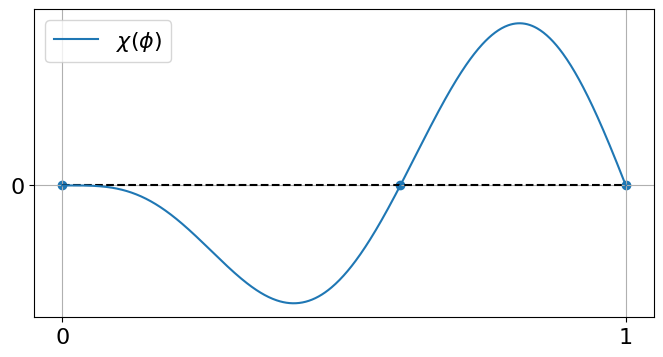
\includegraphics[width=0.77\textwidth]{figures/equilibriums_case_2.png}
	\vspace{-0.3cm}
	\caption{Поведение функции $\chi(\phi)$, случай <<среднего напряжения>>.}
	\label{fig:equilibriums_case_2}
	\vspace{0.7cm}
	
	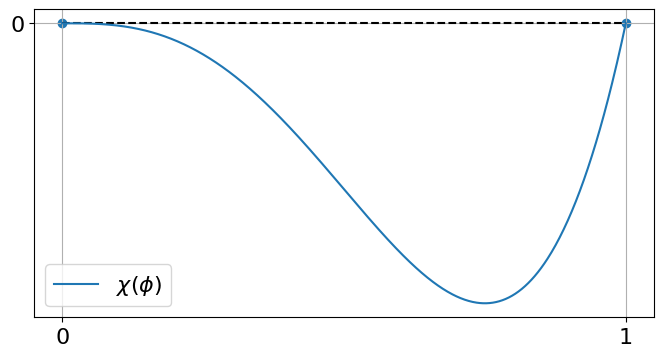
\includegraphics[width=0.77\textwidth]{figures/equilibriums_case_3.png}
	\vspace{-0.3cm}
	\caption{Поведение функции $\chi(\phi)$, случай <<сильного напряжения>>.}
	\label{fig:equilibriums_case_3}
\end{figure}

%!TEX root = ../main.tex

\section{Finite difference scheme}
\label{sec:differential_scheme}

In this section we present finite-difference scheme for solution of
the equation~\eqref{eq:one_dim} in the domain~$[0, W]_x \times [0,
+\infty)_t$
subjected to initial conditions~\eqref{eq:one_dim_initial} and boundary conditions~\eqref{eq:one_dim_marginal}.

Consider regular mesh with time step~$\tau$ and
spatial mesh step size~$h$. Let~$W = Nh$ with $N$ being number of
nodes. Nodes of spatiotemporal grid are given by~$(jh, k \tau)$,
$j = \overline{0, N}$, $k \in \Natural_0$. Define by~$\phi_j^k$
a value of mesh function~$\phi$ at the node~$(jh, k \tau)$.
Then the finite-difference approximations read
\begin{equation}
  \cfrac{1}{m} \difftau{\phi} = \half K_\phi^2 \epsilon'(\phi_j^k) + \cfrac{\Gamma}{l^2} f'(\phi_j^k) + \cfrac{\Gamma}{2} \diffhh{\phi} \tpoint
  \label{eq:subtractive}
\end{equation}
or, in the explicit form,
\begin{gather}
  \begin{aligned}
    \phi_j^{k + 1} = \phi_j^k + m \tau \left( \half K_\Phi^2 \epsilon'(\phi_j^k) + \cfrac{\Gamma}{l^2} f'(\phi_j^k) + \cfrac{\Gamma}{2} \diffhh{\phi} \right), \\ j = \overline{1, N - 1}, \quad k \in \Natural_0 \tsemicolon
  \end{aligned}
  \label{sch:transition} \\
  \phi_j^0 = \phi_0(jh); \quad \phi_0^k = \phi_l(k \tau); \quad \phi_N^k = \phi_r(k \tau) \tpoint
  \label{sch:borders}
\end{gather}

It is easy to see the scheme is of the first order of approximation in
time and second order approximation in spatial terms.

To study properties of the scheme~\eqref{sch:transition}, \eqref{sch:borders}
the linear theory can be used (see, e.g.,
\cite[Chapter~10]{bahvalov_computational_methods}
or~\cite[Chapter~IX]{kalitkin_computational_methods}).
The central result of the theory states, in a somewhat simplified
form, that if a finite-difference scheme is stable and approximate
continuous problem, then solution of the finite-dimensional problem
converges to the solution of the continuous one with the order
not lower then order of approximation.

To apply this result for the nonlinear setting~\eqref{sch:transition}, \eqref{sch:borders} at
hand we proceed in the following way:
(i) linearize equation~\eqref{eq:subtractive}
for fixed~$\phi$, and then (ii) apply spectral stability argument~\cite{bahvalov_computational_methods} to the
derived linearized equation. As stability criteria will be
satisfied for the linearized equation, it should be expected for the
complete, nonlinear, problem. In this case convergence of the
approximate solution should be expected as well~--- since
the finite-difference problem is stable and approximate the continuous
one.
The results of such non-rigorous analysis will be further confirmed by
numerical computations in the fully nonlinear setting.


\subsection{Stability estimate}

In this section we derive  stability condition for
finite-difference scheme~\eqref{sch:transition}, \eqref{sch:borders}
using the so called principal of the ``frozen coefficients''
(see, e.g.,~\cite{bahvalov_computational_methods}).
Let~$\phi_j^k$ and~$\phi_j^k + \delta_j^k$ be solutions of the
finite-difference equation~\eqref{eq:subtractive}.
Substitute~$\phi_j^k + \delta_j^k$ into~\eqref{eq:subtractive} to obtain:
\begin{multline*}
  \cfrac{1}{m} \cfrac{(\phi_j^{k + 1} + \delta_j^{k + 1}) - (\phi_j^k + \delta_j^k)}{\tau} = \half K_\Phi^2 [\epsilon'(\phi_j^k) + \epsilon''(\phi_j^k) \delta_j^k + o(\delta_j^k)] + \\ + \cfrac{\Gamma}{l^2} [f'(\phi_j^k) + f''(\phi_j^k) \delta_j^k + o(\delta_j^k)] + \cfrac{\Gamma}{2} \cfrac{(\phi_{j + 1}^k + \delta_{j + 1}^k) - 2 (\phi_j^k + \delta_j^k) + (\phi_{j - 1}^k + \delta_{j - 1}^k)}{h^2} \tpoint
\end{multline*}
Linearizing this equation around~ $\phi_j^k = P$, assuming that
perturbations~$\delta_j^k$ are small, and taking into account
that~$\phi_j^k$ is a solution of the finite-difference problem, one
arrives to:
\begin{equation}
  \delta_j^{k + 1} = \delta_j^k + m \tau \left( \half K_\Phi^2 \epsilon''(P) \delta_j^k + \cfrac{\Gamma}{l^2} f''(P) \delta_j^k + \cfrac{\Gamma}{2} \diffhh{\delta} \right) \tpoint
  \label{eq:scheme_variation}
\end{equation} 

We now apply spectral stability analysis for the derived equation for
perturbations.
Let~$\delta_j^k = \lambda(\theta)^k \cdot \exp(\imath j \theta)$, $\imath^2 = -1$.
Substituting this representation into~\eqref{eq:scheme_variation} one obtains:
$$\lambda(\theta) = 1 + m \tau \left( \half K_\Phi^2 \epsilon''(P) + \cfrac{\Gamma}{l^2} f''(P) + \cfrac{\Gamma}{2} \cfrac{\exp(\imath \theta) - 2 + \exp(-\imath \theta)}{h^2} \right) \tcomma$$
or
\begin{equation}
  \lambda(\theta) = 1 + m \tau \left( \half K_\Phi^2 \epsilon''(P) + \cfrac{\Gamma}{l^2} f''(P) - \cfrac{2 \Gamma}{h^2} \sin^2 \cfrac{\theta}{2} \right) \tpoint
  \label{eq:spectral}
\end{equation}

According to the spectral stability argument, a time
step~$\tau = \tau(h)$ provides stability of the scheme in the
domain~$[0, W]_x \times [0, T]_t$ with~$T<+\infty$ as~$\tau, h \to 0$, if there
exists~$C > 0$, such that for an arbitrary~$\theta$ it
holds~$|\lambda(\theta)| \leqslant \exp(C\tau)$.  Note that here it is
also possible to use more strict condition~$|\lambda(\theta)| \leqslant 1 + C\tau$.
If for an arbitrary~$\theta$ it holds~$|\lambda(\theta)| \leqslant 1$,
then stability will be provided also for unbounded time interval, i.e.,
for~$[0, W]_x \times [0, +\infty)_t$.
Strictly speaking, spectral argument does not provide sufficient
stability condition however it should be expected in practice.

First, consider expression~\eqref{eq:spectral} for~$P=0$.
We have~$f''(0) = 0$, $\epsilon''(0) = 0$ and equation~\eqref{eq:spectral}
takes a form of
$$\lambda(\theta) = 1 - \cfrac{2 \tau m \Gamma}{h^2} \sin^2 \cfrac{\theta}{2} \tpoint$$
Hence, for an arbitrary~$\theta$ it holds~$|\lambda(\theta)| \leqslant 1$,
if and only if
\begin{equation}
  \tau \leqslant \cfrac{h^2}{m \Gamma} \tpoint
  \label{cond:spectral_0}
\end{equation}
As condition~\eqref{cond:spectral_0} is satisfied one can expect stability of the scheme
when solution describes completely damaged, or closed to it, state~$\phi\approx0$
in the domain~$[0, W]_x \times [0, +\infty)_t$.

Note that under condition~\eqref{cond:spectral_0} one also can expect stable computations
for~$[0, W]_x \times [0, T]_t$ for an arbitrary value~$P \in [0, 1]$.
In this case it holds
$$
|\lambda(\theta)| \leqslant \left| 1 - \cfrac{2 \tau m \Gamma}{h^2} \sin^2 \cfrac{\theta}{2} \right| + m \tau \left| \half K_\Phi^2 \epsilon''(P) + \cfrac{\Gamma}{l^2} f''(P) \right| \leqslant 1 + m \tau \left| \half K_\Phi^2 \epsilon''(P) + \cfrac{\Gamma}{l^2} f''(P) \right| \tpoint
$$
Hence, there exists~$C$ such that
$|\lambda(\theta)| \leqslant 1 + C \tau$ holds,~--- since~$\epsilon''(\phi)$ and~$f''(\phi)$
are continuous on~$[0, 1]$.
It should be noted that despite such versatility, estimate~\eqref{cond:spectral_0}
is poorly applicable in practice and requires clarification, which will be done later.

We now consider expression~\eqref{eq:spectral} at the value~$P=1$.
It holds~$f''(1) < 0$, $\epsilon''(1) > 0$.
Note that for~$(K_\Phi^2 / 2) \epsilon''(1) + (\Gamma / l^2) f''(1) \leqslant 0$
it is possible it is possible to achieve~ $|\lambda(\theta)| \leqslant 1$
having demanded, similar to~\eqref{cond:spectral_0}, $\tau \leqslant h^2 / (2m \Gamma)$
and sufficiently small values of~$\tau$.
Substituting~$f''(1) = -12, \; \epsilon''(1) = 12 \epsilon_0 / (1 + \delta)^2$ (see~\eqref{eq:epsilon_derivatives}),
one arrives to
\begin{equation}
  \cfrac{K_\Phi^2 l^2 \epsilon_0}{2 \Gamma (1 + \delta)^2} \leqslant 1 \tpoint
  \label{cond:spectral_possible_1}
\end{equation}

So, under condition~\eqref{cond:spectral_possible_1}, it is expected
existence of such values of~$\tau$ и $h$,
that difference scheme is stable for~$\phi \approx 1$
and~$T=+\infty$.
Naturally the condition~\eqref{cond:spectral_possible_1}
is equivalent to the stability condition~\eqref{cond:equilibrium_1_stable}
for equilibrium state~$\phi \equiv 1$ of the equation~\eqref{eq:one_dim}.

\subsection{Improved stability estimate}

In the previous section form the analysis of equation~\eqref{eq:spectral}
it was derived stability condition~\eqref{cond:spectral_0}
for finite-difference scheme~\eqref{sch:transition} and~\eqref{sch:borders} for~$\phi \approx 0$.
The assumption of its usefulness is based on the fact that typical ``'natural'' solution of the model
will has a form of the transition process from the undamaged state~$\phi=1$ to the completely
damaged state~$\phi=0$ occurring in a finite time interval and then infinitely long staying in the
damaged state~$\phi \approx 0$.


However the performed analysis of the equation~\eqref{eq:spectral}
is not sufficient at~$\phi = 0$. Indeed, it was used that at~$\phi=0$,
$\epsilon''(0) = 0$ (see expression~\eqref{eq:epsilon_derivatives}),~---
but it was not accounted that~$\epsilon''(\phi)$ growth fast and reaches
large values  for small values of~$\delta\approx 0$,
see Fig.~\ref{fig:eps_phi_phi}.
This means that the equations of the model are stable at~$\phi=0$,
but can be unstable in the small neighbourhood of~$\phi=0$.
Such situation is not satisfactory and we now try to improve
the obtained stability estimates.
%
\begin{figure}[!t]
	\centering
	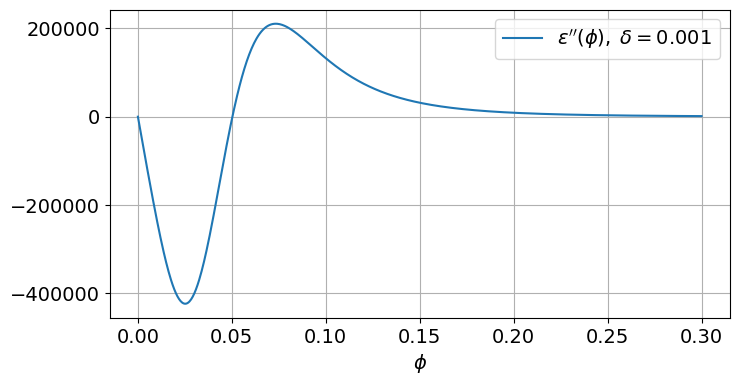
\includegraphics[width=\textwidth]{figures/eps_phi_phi.png}
	\vspace{-0.7cm}
	\caption{Typical behavior of~$\epsilon''(\phi)$ in the vicinity of~$0$.}
	\label{fig:eps_phi_phi}
\end{figure}

To proceed let us estimate extremums of~$\epsilon''(\phi)$ in the neighbourhood of~$0$.
First, find zeros of~$\epsilon'''(\phi)$. We have
\begin{equation}
	\epsilon''' = \epsilon_0 \cfrac{-6 (f')^3 + 6 (f + \delta) f' f'' - (f + \delta)^2 f'''}{(f + \delta)^4},
	\label{eq:epsilon_phi_phi_phi}
\end{equation}
form where:
$$\epsilon'''(\phi) = -6 (f')^3 + 6 (f + \delta) f' f'' - (f + \delta)^2 f''' = 0 \tcomma$$
or, taking~\eqref{eq:epsilon} into account:
$$-3 \cdot 12^2 (1 - \phi)^3 + 36 \left(4 - 3\phi + \cfrac{\delta}{\phi^3} \right)(1 - \phi)(2 - 3\phi) - \left(4 - 3 \phi + \cfrac{\delta}{\phi^3} \right)^2 (1 - 3 \phi) = 0 \tpoint$$

Let~$\delta_n \to +0$ and~$\phi_n \to +0$ such that~$\delta_n / \phi_n^3$ is bounded.
Then:
\begin{gather*}
	-3 \cdot 12^2 \cdot 1^3 + 36 \left(4 + \cfrac{\delta_n}{\phi_n^3} \right) \cdot 1 \cdot 2 - \left(4 + \cfrac{\delta_n}{\phi_n^3} \right)^2 \cdot 1 \to 0 \tcomma \\
	\left(4 + \cfrac{\delta_n}{\phi_n^3} \right)^2 - 72 \left(4 + \cfrac{\delta_n}{\phi_n^3} \right) + 3 \cdot 12^2 \to 0 \tpoint
\end{gather*}
Hence, a sequence~$4 + \delta_n / \phi_n^3$ has not more than two partial limits~$\xi_+$ and~$\xi_-$~---
which are zeros of the equation~$\xi^2 - 72 \xi + 432 = 0$.
To the first zero~$\xi_+ = 36 + 12 \sqrt{6}$ it corresponds
$$\phi_+ = \cfrac{1}{\sqrt[3]{32 + 12 \sqrt{6}}} \sqrt[3]{\delta_n} \approx \cfrac{1}{3.945} \sqrt[3]{\delta_n} \tsemicolon$$
to the second zero~$\xi_- = 36 - 12 \sqrt{6}$ it corresponds
$$\phi_- = \cfrac{1}{\sqrt[3]{32 - 12 \sqrt{6}}} \sqrt[3]{\delta_n} \approx \cfrac{1}{1.376} \sqrt[3]{\delta_n} \tpoint$$

From here it can be seen that for~$\delta \to +0$ the function~$\epsilon'''(\phi)$ has two zeros in the neighbourhood of~$0$:
\begin{equation}
  \phi_{\pm} = \cfrac{1}{\sqrt[3]{32 \pm 12 \sqrt{6}}} \sqrt[3]{\delta} [1 + o(1)] \tpoint
  \label{eq:epsilon_phi_phi_phi_roots}
\end{equation}

We now estimate~$\epsilon''(\phi)$ at~$\phi_{\pm}$  for~$\delta \to +0$. Let~$\phi = (1 / c) \sqrt[3]{\delta}$, $c \in \Real$.
Then:
$$\epsilon'' = \epsilon_0 \cfrac{24 c^5 (8 - c^3)}{(4 + c^3)^3} \delta^{-5 / 3} [1 + o(1)],$$
and:
\begin{equation}
  \epsilon''(\phi_+) \approx -4.378 \epsilon_0 \delta^{-5 / 3}; \quad \epsilon''(\phi_-) \approx 2.216 \epsilon_0 \delta^{-5 / 3} \tpoint
  \label{est:epsilon_phi_phi_bounds}
\end{equation}
The derived estimates are shown as black dashed lines on Fig.~\ref{fig:eps_phi_phi_multiplied}.

\begin{figure}[!t]
	\centering
	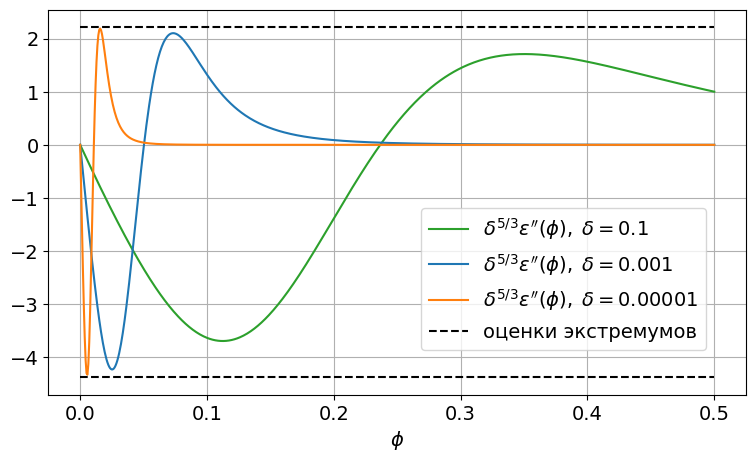
\includegraphics[width=\textwidth]{figures/eps_phi_phi_multiplied.png}
	\caption{Qualitative behavior of~$\delta^{5 / 3} \epsilon''(\phi)$ for small values of~$\delta$.}
	\label{fig:eps_phi_phi_multiplied}
\end{figure}

Now, to derive new stability estimate we consider equation~\eqref{eq:spectral} at~$\phi = \phi_+$.
Note that~$\epsilon''(\phi_+) \approx -4.4 \epsilon_0 \delta^{-5 / 3}$.
The term inside braces in~\eqref{eq:spectral} is negative since
$\delta$ is small and~$\epsilon''(\phi_+)$ is negative and large in its absolute value.
Therefore~$f''(\phi_+) > 0$ can be estimated as~$0$~--- such estimate makes inequality stronger.
Then from inequality~\eqref{eq:spectral} it follows that 
$$\lambda(\theta) = 1 + m \tau \left( -\cfrac{2.2 K_\Phi^2 \epsilon_0}{\delta^{5 / 3}} - \cfrac{2 \Gamma}{h^2} \sin^2 \cfrac{\theta}{2} \right) \tpoint$$
Condition~$|\lambda(\theta)| \leqslant 1$ is satisfied for an arbitrary~$\theta$, if and only if
\begin{equation}
  \tau \leqslant \cfrac{1}{m} \left( \cfrac{1.1 K_\Phi^2 \epsilon_0}{\delta^{5 / 3}} + \cfrac{\Gamma}{h^2} \right)^{-1} \tpoint
  \label{cond:spectral_better_theoretical}
\end{equation}

Numerical experiments described in the next sections indicates that
more strong version of the estimate~\eqref{cond:spectral_better_theoretical} is also valid
(note the doubled denominator):
%
\begin{equation}
  \tau \leqslant \cfrac{1}{2m} \left( \cfrac{K_\Phi^2 \epsilon_0}{\delta^{5 / 3}} + \cfrac{\Gamma}{h^2} \right)^{-1} \tpoint
  \label{cond:spectral_better}
\end{equation}

Finally, more simple estimate not weaker then~\eqref{cond:spectral_better} is:
\begin{equation}
  \tau \leqslant \cfrac{1}{4m} \min \left(\cfrac{\delta^{5 / 3}}{K_\Phi^2 \epsilon_0}, \; \cfrac{h^2}{\Gamma} \right) \tpoint
  \label{cond:spectral_better_simpler}
\end{equation}

Note that the derived stability estimate~\eqref{cond:spectral_better}
for finite-difference scheme~\eqref{sch:transition},\eqref{sch:borders}
includes all the parameters of the equation~\eqref{eq:one_dim}, except~$l$.
Notably, this is the only parameter of the model which has somehow artificial nature and can not be
related directly to the underlying physics.

\endinput
% EOF

%!TEX root = ../main.tex

\section{Численное исследование}

Была написана программа, реализующая разностную схему \eqref{sch:transition}, \eqref{sch:borders}. С помощью моделирования проверим полученные ранее теоретические результаты, а именно: устойчивость и сходимость схемы при выполнении условия устойчивости \eqref{cond:spectral_better}, а также свойства положений равновесия системы, описанные в разделе \ref{sec:theoretical_analysis}. Помимо этого проверим поведение полной свободной энергии системы при моделировании.


\subsection{Вычислительный эксперимент: устойчивость}

Зафиксируем параметры уравнения \eqref{eq:one_dim}:
\begin{equation}
	\epsilon_0 = 0.2, \; \delta = 0.04, \; l = 1.0, \; \Gamma = 1.0, \; m = 0.5, \; K_\Phi = 4.8 \tpoint
	\label{exp:parameters}
\end{equation}
Перед нами случай <<сильного напряжения>> (см. выражение~\eqref{char:equilibriums}).

Моделируем решение в области 
\begin{equation}
	\clOmega = [0, W]_x \times [0, T]_t, \; W = 5, \; T = 1 \tpoint
	\label{exp:set}
\end{equation}

Зададим следующие краевые условия:
\begin{equation}
\begin{gathered}
	\phi(0, t) = 1, \; \phi(W, t) = 1 \tcomma \\
	\phi(x, 0) = \phi_0(x) = \begin{cases}
		1, \; \text{если} \; x \leqslant 2.25 \; \text{или} \; x \geqslant 2.75 \tsemicolon \\
		1 - 0.025 \cdot [1 + \cos(4 \pi x)], \; \text{если} \; 2.25 < x < 2.75 \tpoint
	\end{cases}
\end{gathered} \label{exp:borders}
\end{equation}
Обратим внимание, что $\phi_0(x)$ дважды дифференцируема всюду, кроме конечного числа точек, с ограниченной второй производной.

Обозначим $N_x$ число отрезков разбиения $[0, W]_x$ (узлов, соответственно, $N_x + 1$); $N_t$ -- число отрезков разбиения $[0, T]_t$. $h = W / N_x, \; \tau = T / N_t$.

\begin{figure}[!tp]
	\centering
	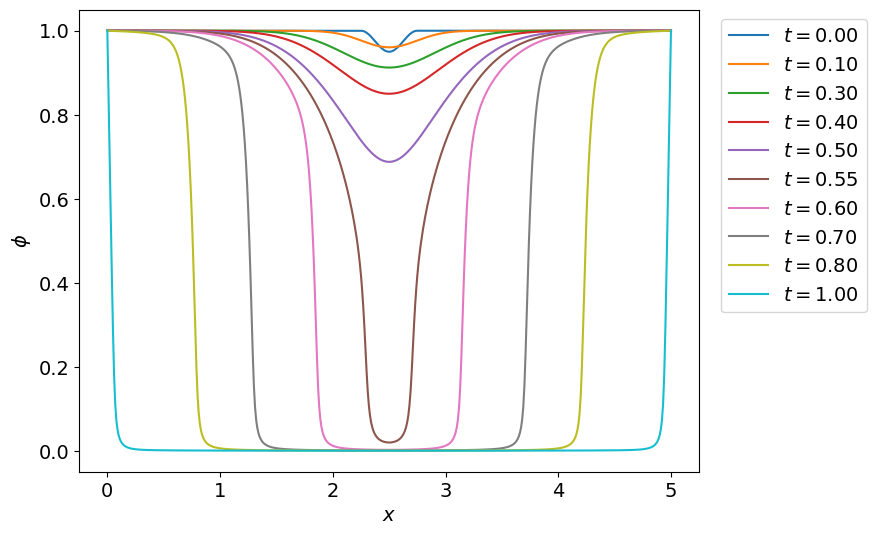
\includegraphics[width=\textwidth]{figures/typical_solution.png}
	\vspace{-0.8cm}
	\caption{Типичное решение задачи, $N_x = 10^3, \; N_t = 10^5$.}
	\label{fig:typical_solution}
\end{figure}

Для начала посмотрим на типичное решение исследуемой задачи (рис.~\ref{fig:typical_solution}). Видно постепенное развитие канала электрического пробоя (разрушение среды) из небольшого начального возмущения фазового поля $\phi$ неповрежденной среды. Примерно в момент времени $t = 0.55$ канал пробоя <<прорастает насквозь>>, а именно, $\phi$ вблизи точки $x = 2.5$ приближается к нулевому значению. Обратим внимание, что в период времени $t \in (0.3, \; 0.55)$ канал пробоя (область, где $\phi$ существенно отличается от $1$) практически не растет в ширину, а при $t > 0.55$, напротив, растет в ширину почти с постоянной скоростью.

Проверим полученную в предыдущем разделе оценку \eqref{cond:spectral_better} устойчивости разностной схемы. Будем считать, что в вычислительном эксперименте схема неустойчива, если программа завершилась с ошибкой: произошло деление на~$0$ (в формуле \eqref{eq:epsilon} функции $\epsilon(\phi)$ при $f(\phi) = -\delta$) или значения $\phi$ ушли на бесконечность (переполнился тип double). Будем перебирать $N_x$ и $N_t$, запоминая пары соседних точек, в одной из которых устойчивость есть, а в другой нет. Так получим опытную оценку устойчивости схемы. Отобразим ее на графике вместе с оценкой \eqref{cond:spectral_better} (рис. \ref{fig:stability_bounds}).

Эксперимент показывает, что оценка \eqref{cond:spectral_better} удачна: она примерно повторяет контур опытной оценки, к тому же ее график лежит выше, то есть она имеет некоторый <<запас>> до момента, когда в программе возникает ошибка. Именно ради этого <<запаса>> знаменатель исходной оценки  \eqref{cond:spectral_better_theoretical} был удвоен.

\begin{figure}[!tp]
	\centering
	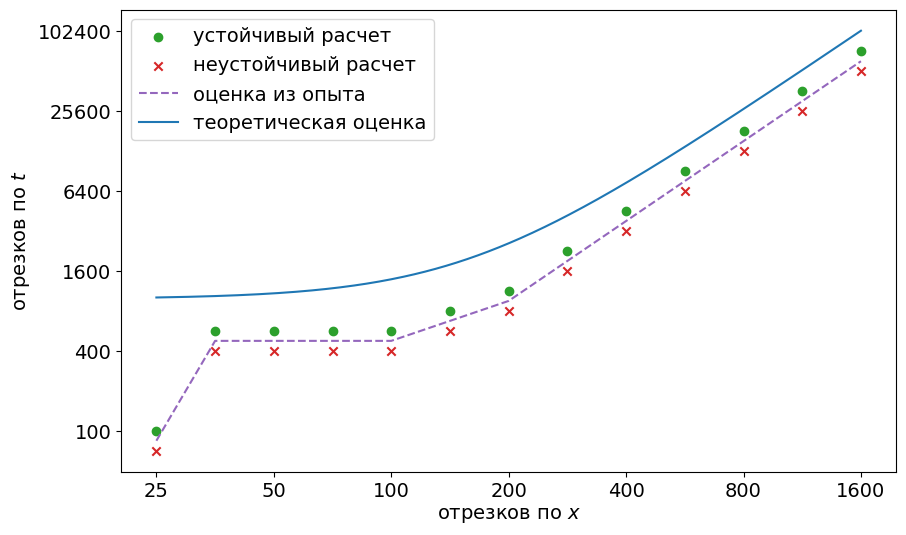
\includegraphics[width=\textwidth]{figures/stability_bounds.png}
	\vspace{-0.7cm}
	\caption{Теоретическая и опытная оценки устойчивости разностной схемы.}
	\label{fig:stability_bounds}
\end{figure}


\subsection{Вычислительный эксперимент: сходимость}

Аппроксимация разностной схемой \eqref{sch:transition}, \eqref{sch:borders} дифференциальной задачи \eqref{eq:one_dim}, \eqref{eq:one_dim_initial}, \eqref{eq:one_dim_marginal} очевидна; для устойчивости схемы в ходе нестрогого анализа получено условие \eqref{cond:spectral_better}, применимое на практике. Теперь экспериментально проверим сходимость.

На множестве $C_2(\clOmega)$ дважды непрерывно дифференцируемых функций в замкнутой области $\clOmega = [0, W]_x \times [0, T]_t$ рассмотрим следующие нормы: непрерывную $\enorm_C$ и $L_2$-норму $\enorm_2$.
$$\norm{f}_C = \max \limits_{(x, t) \in \clOmega} |f(x, t)|; \qquad \norm{f}_2 = \sqrt{\int \limits_{\clOmega} f^2(x, t) dx dt} \tpoint$$

Теперь рассмотрим регулярную сетку $\Omega_{h, \tau} \subset \clOmega$ с некоторой зависимостью $\tau = \tau(h)$. Ограничивая функции из $C_2(\Omega)$ на сетке $\Omega_h = \Omega_{h, \tau(h)}$, получаем множество $C_2(\clOmega)_h$ сеточных функций.

На множестве $C_2(\clOmega)_h$ сеточных функций введем нормы, согласованные с $\enorm_C$ и $\enorm_2$:
$$\norm{f_j^k}_C = \max \limits_{(j, k) \in \Omega_h} |f_j^k|; \qquad \norm{f_j^k}_2 = \sqrt{h \tau \sum \limits_{(j, k) \in \Omega_h} (f_j^k)^2} \tpoint$$

Перейдем к вычислительному эксперименту. Сходимость будем проверять по описанным выше нормам $\enorm_C$ и $\enorm_2$ на множестве сеточных функций. Так как аналитическое решение дифференциальной задачи не известно, будем сравнивать ряд результатов на все более мелких сетках по норме с лучшим результатом в ряду. При сравнении функцию на более мелкой сетке ограничиваем на более крупной, игнорируя часть узлов.

Зафиксируем ранее использовавшиеся параметры уравнения \eqref{exp:parameters}, \eqref{exp:set}; зададим краевые условия \eqref{exp:borders}. Положим $N_x = W / h$ -- число отрезков разбиения по $x$, $N_t = T / \tau$ -- по $t$.

Во всех описанных далее вариантах расчетов соблюдается условие устойчивости~\eqref{cond:spectral_better}.

Для начала зафиксируем $N_x = 200$ и будем перебирать $N_t$, каждый раз увеличивая его вдвое. Сравнение по нормам с результатом при $N_t = 204800$ изображено на рис. \ref{fig:convergence_fixed_nx}. Разностная схема имеет первый порядок аппроксимации по $t$; опыт показывает первый порядок сходимости $\bigO (\tau)$.

Зафиксируем $N_t = 204800$ и будем перебирать $N_x$, каждый раз увеличивая его вдвое. Сравнение по нормам с результатом при $N_x = 1600$ изображено на рис. \ref{fig:convergence_fixed_nt}. Разностная схема имеет второй порядок аппроксимации по $x$; опыт показывает второй порядок сходимости $\bigO (h^2)$.

\begin{figure}[!tp]
	\centering
	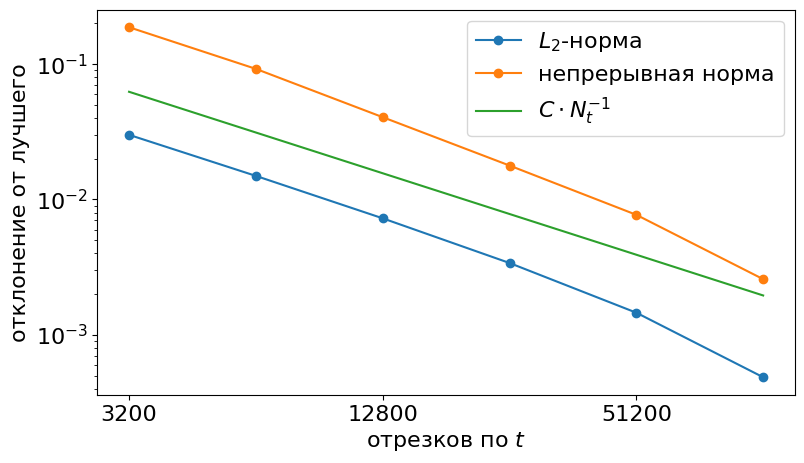
\includegraphics[width=0.72\textwidth]{figures/convergence_fixed_nx.png}
	\vspace{-0.2cm}
	\caption{Ошибка решения по норме при фиксированном $N_x = 200$.}
	\label{fig:convergence_fixed_nx}
	\vspace{0.6cm}
	
	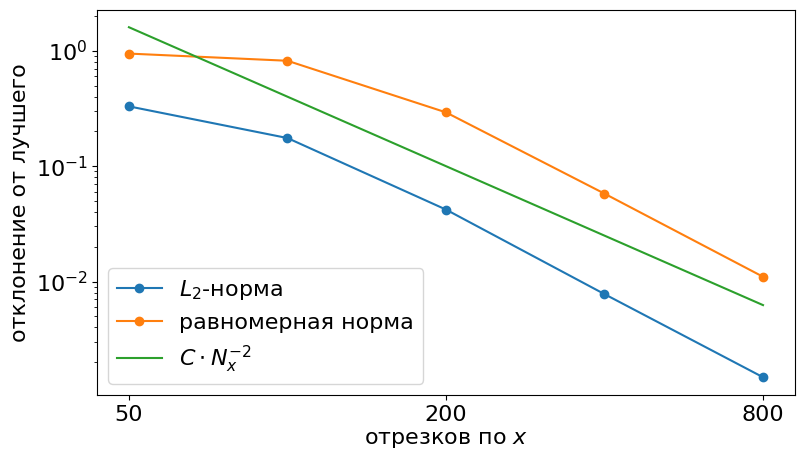
\includegraphics[width=0.72\textwidth]{figures/convergence_fixed_nt.png}
	\vspace{-0.2cm}
	\caption{Ошибка решения по норме при фиксированном $N_t = 204800$.}
	\label{fig:convergence_fixed_nt}
	\vspace{0.6cm}
	
	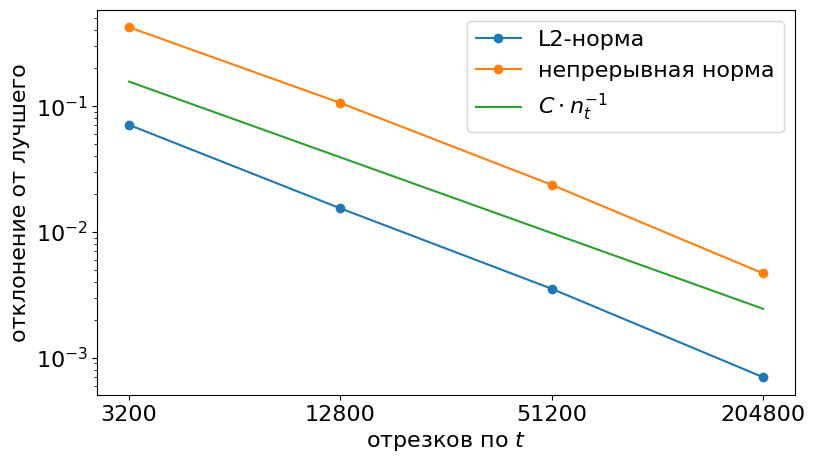
\includegraphics[width=0.72\textwidth]{figures/convergence_connected.png}
	\vspace{-0.2cm}
	\caption{Ошибка решения по норме при $N_t = 0.08 \cdot N_x^2$.}
	\label{fig:convergence_connected}
\end{figure}

Теперь свяжем $N_x$ и $N_t$ уравнением, так чтобы при $h, \tau \to 0$ выполнялось условие устойчивости \eqref{cond:spectral_better}. При выбранных параметрах модели подойдет $N_t = 0.08 \cdot N_x^2$. Аналогично проведем сравнение ряда измерений по норме с лучшим (рис. \ref{fig:convergence_connected}). Как и ожидалось, измерения показывают сходимость $\bigO (\tau + h^2) = \bigO (\tau)$ первого порядка по времени при выбранном уравнении связи.

В первых двух опытах, без стремления обоих шагов сетки к $0$, последовательности сеточных функций имели неясный предел. В третьем же, если принять предположение об устойчивости разностной схемы, сеточные функции сходятся к решению дифференциальной задачи \eqref{eq:one_dim}, \eqref{eq:one_dim_initial}, \eqref{eq:one_dim_marginal}.


\subsection{Вычислительный эксперимент: \\ положения равновесия}

Ранее были исследованы положения равновесия уравнения \eqref{eq:one_dim} вида $\phi \equiv C$. Их количество и устойчивость определяется значением выражения \eqref{char:equilibriums} (обозначено $\xi$). Проверим этот результат экспериментально.

Зададим модели параметры \eqref{exp:parameters}, \eqref{exp:set}, $K_\Phi$ определим позже. В качестве начального условия берем возмущенное положение равновесия: $\phi(x, 0) = C + A \cos(\omega x); \; \phi(0, t) = \phi(0, 0), \; \phi(W, t) = \phi(W, 0)$. Амплитуда $A$ мала, порядка~$0.01$. $N_x = 800, \; N_t = 51200$.

Если положение равновесия устойчиво, то при любом $\omega$ возмущение угасает; если неустойчиво, то существует некоторое $\omega_0$, такое что при $\omega < \omega_0$ возмущение растет.

Положим $K_{\Phi, 1} = 0, \; K_{\Phi, 2} = 1.1, \; K_{\Phi, 3} = 4.8$. Было задано $\delta = 0.04$. В таком случае $\xi_1 = 0 < \delta^2, \; \xi_2 = 0.121 \in (\delta^2, (1 + \delta)^2), \; \xi_3 = 2.304 > (1 + \delta)^2$.

Вначале рассмотрим $K_{\Phi, 1} = 0, \; \xi_1 < \delta^2$ -- случай <<слабого напряжения>>. Система имеет два положения равновесия: $\phi \equiv 0$ неустойчивое, $\phi \equiv 1$ устойчивое. На рис. \ref{fig:equilibrium_1_0}, \ref{fig:equilibrium_1_1} видно теоретически предсказанное поведение возмущенной среды: при $C = 0$ возмущение растет, при $C = 1$ -- затухает. В точке $C = 0$ производная функции $\chi(\phi)$ (см. выражение \eqref{eq:equilibruim_characteristic}) равна $0$, поэтому, чтобы увидеть рост возмущения, приходится брать небольшое $\omega$, обеспечивая небольшое значение $\partflxx{\phi}$. В эксперименте с $\phi \equiv 1$ взято $C = 1 - A$, чтобы значения $\phi$ не превосходили $1$.

\begin{figure}[!t]
	\centering
	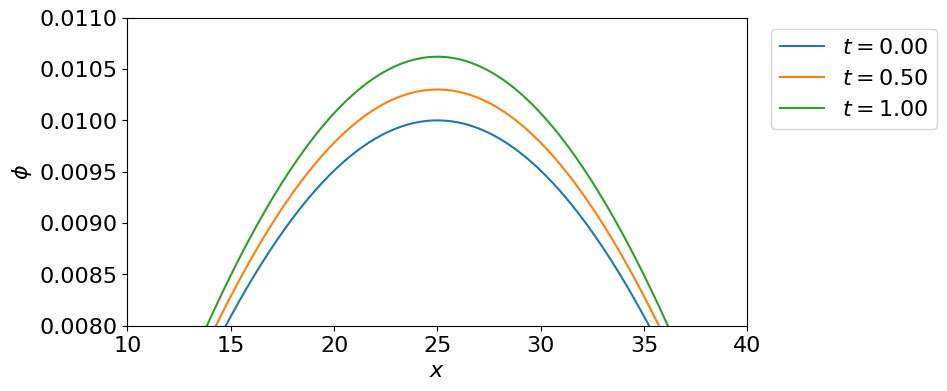
\includegraphics[width=0.9\textwidth]{figures/equilibrium_1_0.png}
	\vspace{-0.3cm}
	\caption{Случай <<слабого напряжения>>: возмущенное положение равновесия $\phi \equiv 0$, неустойчивое.}
	\label{fig:equilibrium_1_0}
	\vspace{0.5cm}
	
	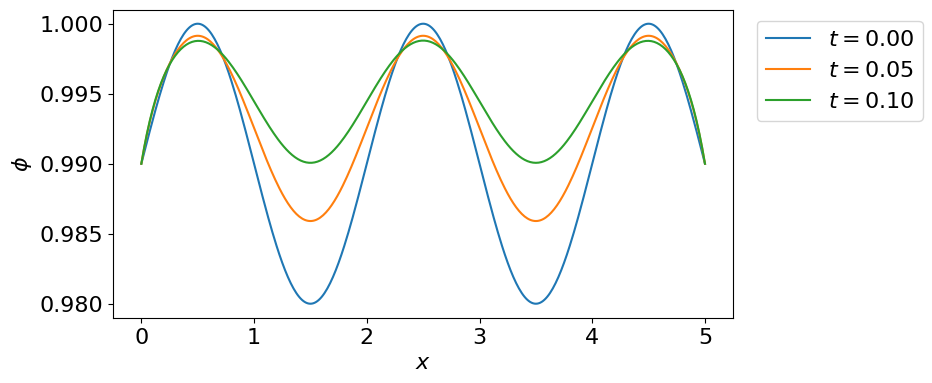
\includegraphics[width=0.9\textwidth]{figures/equilibrium_1_1.png}
	\vspace{-0.3cm}
	\caption{Случай <<слабого напряжения>>: возмущенное положение равновесия $\phi \equiv 1$, устойчивое.}
	\label{fig:equilibrium_1_1}
\end{figure}

Теперь рассмотрим $K_{\Phi, 2} = 1.1, \; \xi_2 \in (\delta^2, (1 + \delta)^2)$ -- случай <<среднего напряжения>>. Система имеет три положения равновесия: $\phi \equiv 0$ устойчивое, $\phi \equiv C_3 \approx 0.5$ неустойчивое ($C_3$ -- корень функции $\chi(\phi)$ в интервале $(0, 1)$), $\phi \equiv 1$ устойчивое. Поведение возмущенной среды изображено на рис. \ref{fig:equilibrium_2_0}, \ref{fig:equilibrium_2_05}, \ref{fig:equilibrium_2_1}, оно соответствует теоретическим результатам.

\begin{figure}[!tp]
	\centering
	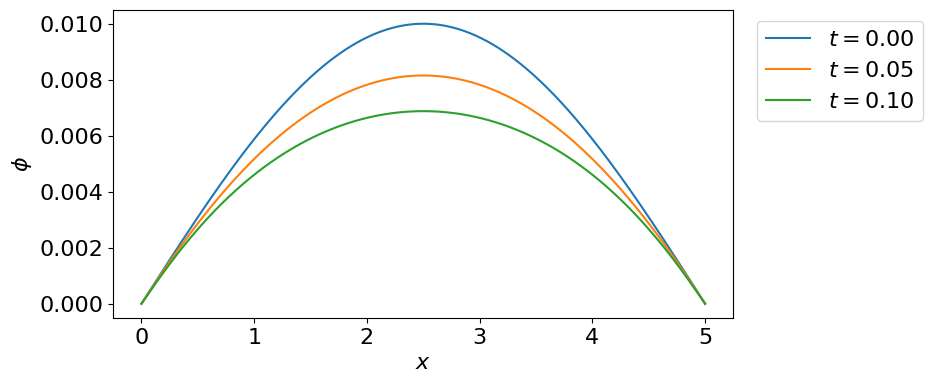
\includegraphics[width=0.9\textwidth]{figures/equilibrium_2_0.png}
	\vspace{-0.3cm}
	\caption{Случай <<среднего напряжения>>: возмущенное положение равновесия $\phi \equiv 0$, устойчивое.}
	\label{fig:equilibrium_2_0}
	\vspace{0.5cm}

	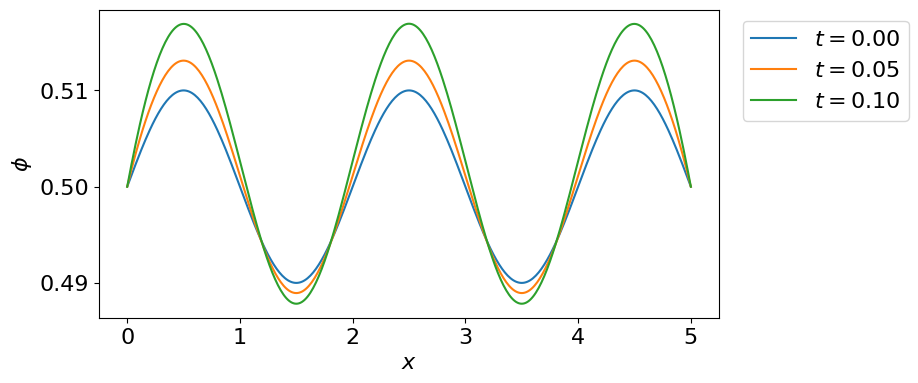
\includegraphics[width=0.9\textwidth]{figures/equilibrium_2_05.png}
	\vspace{-0.3cm}
	\caption{Случай <<среднего напряжения>>: возмущенное положение равновесия $\phi \equiv C_3 \approx 0.5$, неустойчивое.}
	\label{fig:equilibrium_2_05}
	\vspace{0.5cm}
	
	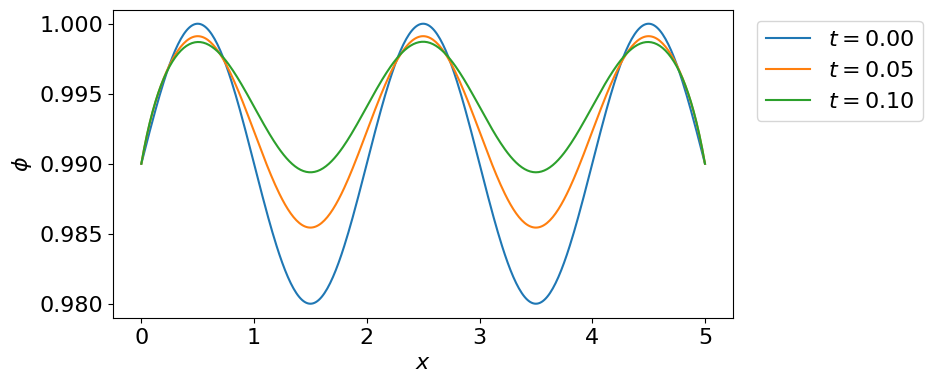
\includegraphics[width=0.9\textwidth]{figures/equilibrium_2_1.png}
	\vspace{-0.3cm}
	\caption{Случай <<среднего напряжения>>: возмущенное положение равновесия $\phi \equiv 1$, устойчивое.}
	\label{fig:equilibrium_2_1}
\end{figure}

Наконец, рассмотрим $K_{\Phi, 3} = 4.8, \; \xi_3 > (1 + \delta)^2$ -- случай <<сильного напряжения>>. Система имеет два положения равновесия: $\phi \equiv 0$ устойчивое, $\phi \equiv 1$ неустойчивое. Поведение возмущенной среды изображено на рис. \ref{fig:equilibrium_3_0}, \ref{fig:equilibrium_3_1}, оно также соответствует теории.

\begin{figure}[!t]
	\centering
	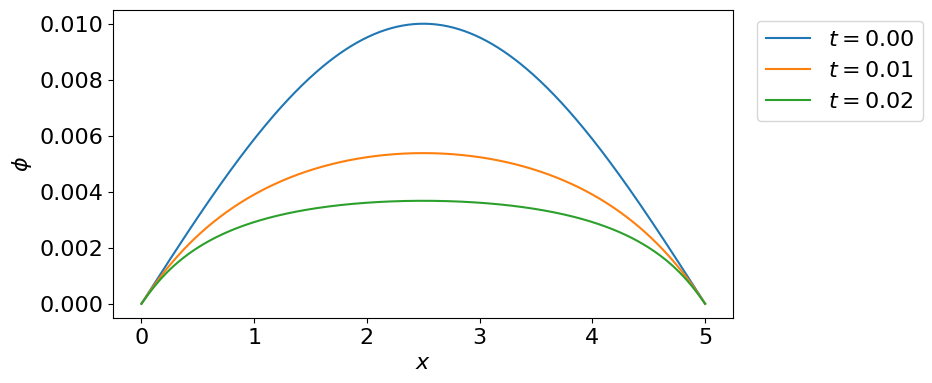
\includegraphics[width=0.9\textwidth]{figures/equilibrium_3_0.png}
	\vspace{-0.3cm}
	\caption{Случай <<сильного напряжения>>: возмущенное положение равновесия $\phi \equiv 0$, устойчивое.}
	\label{fig:equilibrium_3_0}
	\vspace{0.5cm}
	
	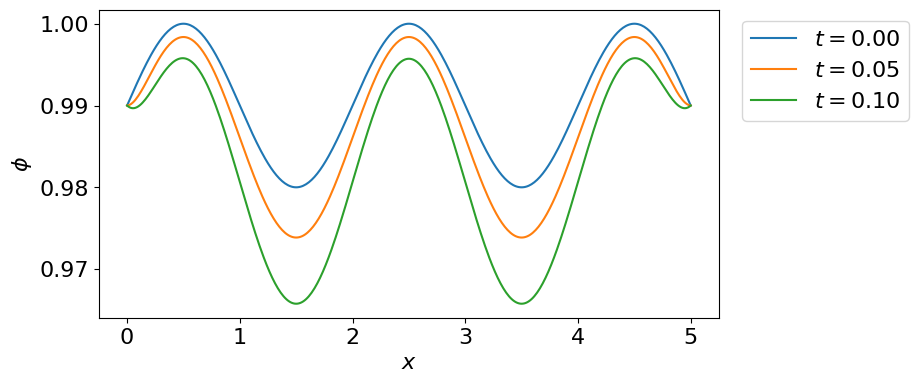
\includegraphics[width=0.9\textwidth]{figures/equilibrium_3_1.png}
	\vspace{-0.3cm}
	\caption{Случай <<сильного напряжения>>: возмущенное положение равновесия $\phi \equiv 1$, неустойчивое.}
	\label{fig:equilibrium_3_1}
\end{figure}


\subsection{Вычислительный эксперимент: свободная энергия}

В рассматриваемой модели введена функция свободной энергии \eqref{eq:energy}, заданная интегралом плотности свободной энергии \eqref{eq:energy_density} по пространству.

Построим график полной свободной энергии системы от времени. Зададим модели параметры \eqref{exp:parameters}, \eqref{exp:set} и краевые условия \eqref{exp:borders}. Ранее мы уже проводили расчеты в этой конфигурации -- графики $\phi$ изображены на рис. \ref{fig:typical_solution}.

Единственное существенное дополнение, требующееся использованной ранее схеме \eqref{sch:transition}, \eqref{sch:borders}, -- вычисление разностной производной $\partial_h \phi_i^j / \partial_h x$. Ограничимся простейшей разностной производной первого порядка, так как искомая величина не влияет на пересчет состояния системы.

Результат вычисления полной свободной энергии $\Pi$ в зависимости от времени изображен на рис. \ref{fig:energy}. Для сравнения с рис. \ref{fig:typical_solution} пунктирными линиями соответствующих цветов отмечены моменты времени. Интересно, что до момента $t = 0.5$ энергия $\Pi$ убывает очень медленно; после, при $t \approx 0.55$, резко падает; затем падение замедляется, и после $t = 0.6$ убывание выравнивается, становясь близким к линейному; так продолжается практически до полного разрушения среды.

\begin{figure}
	\centering
	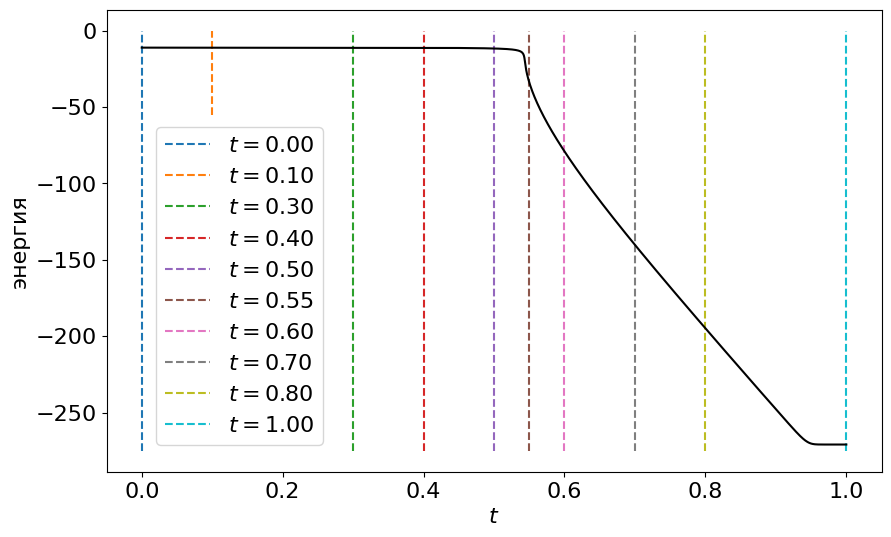
\includegraphics[width=\textwidth]{figures/energy_total.png}
	\vspace{-0.6cm}
	\caption{Поведение полной свободной энергии системы.}
	\label{fig:energy}
\end{figure}

Отметим, что вывод системы уравнений \eqref{eq:Phi}, \eqref{eq:phi} динамики системы из выражений \eqref{eq:energy}, \eqref{eq:energy_density} для свободной энергии означает, что система в ходе эволюции стремится в положение с как можно меньшей свободной энергией. Поэтому для адекватного моделирования системы крайне важно, чтобы полная свободная энергия $\Pi$ не возрастала. Мы не дали этому теоретического обоснования для используемой разностной схемы, однако проверили на опыте. Другими словами, это означает, что при используемом виде краевых условий и параметрах расчета предложенная схема является градиентно-устойчивой.

%!TEX root = ../main.tex

\section{Заключение}

Настоящая работа продолжает исследование, начатое в статье \cite{zipunova_higher_codimension}. Как было отмечено ее авторами, исследование это хотя и проводится для конкретной задачи, но, вероятно, затрагивает вопросы, содержащиеся в методе диффузной границы как таковом. Суть этих вопросов в том, позволяют ли уравнения среды с диффузной границей в своей <<классической>> редакции адекватно описывать включения, по своей природе являющиеся объектами высшей коразмерности. В качестве возможного ответа авторы работы \cite{zipunova_higher_codimension} предлагают определенного вида обобщение исходной модели.

Целью настоящей работы было численно исследовать упомянутое обобщение. В этом достигнуты определенные успехи. С помощью модификации метода конечных объемов преодолены трудности, связанные с необходимостью задавать граничные условия на множествах коразмерности 2 и 3 в трехмерном пространстве и с наличием у функции-решения  особенности в точках этих множеств. Указанный подход существенно не привязан к рассматриваемой модели -- в дальнейшем он может быть использован и в других задачах.

В некоторых случаях при построении разностной схемы возникали фундаментальные препятствия: оказывалось, что необходимых базисных функций попросту не существует. На основании этого выдвинута гипотеза, что в указанных случаях рассматриваемая дифференциальная задача поставлена некорректно и не имеет решения. Рассуждения вполне согласуется с теоретическими результатами работы \cite{zipunova_higher_codimension}. В будущем возможно строгое обоснование представленной гипотезы.

\clearpage
\printbibliography

\clearpage
\tableofcontents

\end{document}

%%%%%%%%%%%%%%%%%%%%%%%%%%%%%%%%%%%%%%%%%%%%%%%%%%%%%%%%%%%%%%%%%%%%%%%%%%%%%%%%